\documentclass[11pt]{report}

%%%%%%%%%%%%%
%% Imports %%
%%%%%%%%%%%%%
\usepackage[a4paper, margin=2cm, top=4cm, bottom=3cm]{geometry}
\usepackage[utf8]{inputenc}
\usepackage[ngerman]{babel}
\usepackage[usenames, dvipsnames]{xcolor}
\usepackage[framemethod=tikz]{mdframed}
\usepackage{listings}
\usepackage{fancyhdr}
\usepackage[acronyms]{glossaries}
\usepackage{tabularx}
\usepackage{booktabs}
\usepackage{cite}
\usepackage{url}
\usepackage{float}
\usepackage{hyperref}

%%%%%%%%%%%%
%% Colors %%
%%%%%%%%%%%%
\definecolor{nordakademie-blue}{RGB}{2,34,94}

%%%%%%%%%%%%%%%%
%% Page Style %%
%%%%%%%%%%%%%%%%
\pagestyle{fancy}
\lhead{\textcolor{nordakademie-blue}{\uppercase{Transferleistung\\ Theorie \& Praxis}}}
\rhead{\textcolor{nordakademie-blue}{
\includegraphics[height=0.85cm,keepaspectratio]{img/NAK-logo}}}
\cfoot{\thepage}
\bibliographystyle{unsrt}
\linespread{1.25}

%%%%%%%%%%%%%%
%% Commands %%
%%%%%%%%%%%%%%
\addto\captionsngerman{\renewcommand{\chaptername}{Abschnitt}}
\newcommand{\inlinecode}{\texttt}
\newcommand*{\SignatureAndDate}[1]{%
    \par\noindent\makebox[2.5in]{\hrulefill}
           \hfill\makebox[2.0in]{\hrulefill}
    \par\noindent\makebox[2.5in][l]{#1}
           \hfill\makebox[2.0in][l]{Datum}
}

%%%%%%%%%%%%%%%%%%%%%%
%% Glossary entries %%
%%%%%%%%%%%%%%%%%%%%%%
\newacronym{bundler}{WAB}{Web Application Bundler}
\newacronym{app}{Web App}{Web Application}
\newacronym{js}{JS}{JavaScript}
\newacronym{html}{HTML}{HyperText Markup Language}
\newacronym{css}{CSS}{Cascading Style Sheets}
\newacronym{cdn}{CDN}{Content delivery network}
\newacronym{hmr}{HMR}{Hot Module Replacement}
\newglossaryentry{cpuTime}
{
  name=CPU-Zeit,
  description={ist die Zeit in welcher ein Prozess Instruktionen auf der CPU ausgeführt hat. Sie unterscheidet sich von der normalen Zeit dahingehend, dass Nutzungen des Prozessors durch andere Prozesse sowie Festplatteninteraktionen nicht mit einfließen\cite{definition:cpuTime}},
  plural=CPU-Zeiten
}
\newglossaryentry{mangling}
{
	name=Mangling,
	description={Komprimierung von Code durch Umbenennung von Variablen, Funktionen, Klassen und Konstanten}
}
\newglossaryentry{loader}
{
	name=Loader,
	description={Abhängigkeit des Build-Tools, welche dafür zuständig ist, einen bestimmten Dateityp zu verarbeiten}
}
\makeglossaries
\makeindex

%%%%%%%%%%%%%%
%% Document %%
%%%%%%%%%%%%%%
\begin{document}

    %%%%%%%%%%%%%%%
    %% Frontpage %%
    %%%%%%%%%%%%%%%
    {\huge Transferleistung 1}
    \vspace{1cm}

    \begin{center}
        \begin{tabularx}{\textwidth}{r|X}
            Matrikelnummer & 8252 \\\midrule
            Thema & Optimierung der Build-Dauer eines Web Application Bundler durch Anpassung der Konfiguration und dessen Auswirkung auf den Entwicklungsprozess \\\midrule
            Studiengang, Zenturie & Angewandte Informatik, A17b\
        \end{tabularx}
    \end{center}
    \pagebreak

    \tableofcontents
    \listoffigures
    \listoftables
    \pagebreak

   	%%%%%%%%%%%%%
    %% Content %%
    %%%%%%%%%%%%%
    \chapter{Einleitung}
    	In der Software-Entwicklung werden häufig Module von anderen Entwicklern in einem Projekt verwendet. Da es in der Web-Entwicklung im Bereich von \Gls{js}, \Gls{html} und \Gls{css} keinen Build-Prozess gibt werden in der klassischen Web-Entwicklung Abhängigkeiten entweder direkt von sogenannten \Glspl{cdn} eingebunden oder manuell heruntergeladen und in das Projekt kopiert.\\
		Alternativ können Abhängigkeiten per Package-Manager (z.B. \emph{npm} oder \emph{yarn}) heruntergeladen werden und in einem Bundling-Prozess mit den vorhandenen Modulen des Projektes zu einer Datei kombiniert werden. Dazu werden \Glspl{bundler} wie zum Beispiel \emph{Webpack} oder \emph{ParcelJS} verwendet.\\
		Zusätzlich zu der Konkatenation von Modulen übernehmen solche Tools die Transformation und Transpilation von Eingabedateien um z.B. Textdateien oder Bilder in den Code zu integrieren, Dateien zu optimieren und komprimieren oder Module, welche in neuen \Gls{js} oder \Gls{css} Versionen geschrieben wurden, in alte Versionen zu übersetzen um Kompatibilität mit älteren Browsern zu gewährleisten.\\
			% Good place to use sources why this is done
		\\
    	Dieses Transferleistung befasst sich mit der Beeinflussbarkeit der Build-Zeit eines \Gls{bundler} durch Anpassungen an der Konfiguration in Bezug auf die Geschwindigkeit des Softwareenwicklungsprozess. In dieser Arbeit werden die folgenden Forschungsfragen näher beleuchtet:
	    	\begin{enumerate}
		    	\item Ist die Build Performance relevant für den Entwicklungsprozess? \label{question0}
		    	\item Welche Faktoren haben eine Auswirkung auf die Dauer des Build? \label{question1}
		    	\item Lassen sich diese Faktoren in einem Software-Projekt beeinflussen? \label{question2}
		    \end{enumerate}
		    
	    \pagebreak

		\section{Relevanz für die PPI AG}
			Bei der PPI AG gibt es mehrere Projekte, welche unter anderem die Entwicklung einer Web-App umfassen. Dies schließt zum Beispiel das Studenten-Verwaltungstool StuMaTo ein, welches der Verwaltung und Verteilung von Aufgaben an die Studenten dient. Dieses Tool wird in der kommenden Praxisphase von einem kleinen Team aus Studenten weiterentwickelt werden, wobei eine direkte Relevanz der Ergebnisse dieser Transferleistung sich positiv auf den Entwicklungsprozess auswirken könnte.
			% TODO Problemstellung verteidigen: Projekttools meist vorgegeben daher Optimierung des Prozess
	
		\section{Relevanz der Build Dauer}
		 	To be done. Beantwortung der Forschungsfrage \ref{question0} % TODO Write this argument

		\section{Methodik}
			Um die Forschungsfrage \ref{question1} zu beantworten ist ein Projekt nötig an dem die Forschung durchgeführt werden kann.
			\subsection{Beispiel-Projekt}
				Im Rahmen dieser Transferleistung wird eine rudimentäre \Gls{app} aufgesetzt, welche sich vom Umfang auf die für den Build Prozess relevanten Kriterien beschränkt und eine Analyse der Faktoren ermöglichen soll, welche einen Einfluss auf die Build Zeit haben.

				\paragraph{Bundling Tool} In vielen Projekten wird die zu nutzende Technologie meist von Projektleitern oder Kunden vorgeschrieben. Entsprechend wurde für dieses Projekt der am weitesten verbreitete\cite{npmtrends:wab} \Gls{bundler} \emph{Webpack} verwendet um eine möglichst einfache Übertragung der Konfigurationsoptionen auf andere Projekte zu ermöglichen.

				\paragraph{React} Bei der Entwicklung von \Glspl{app} werden häufig Frameworks wie z.B. React, Angular oder VueJS verwendet. In diesem Projekt wird \emph{React} aufgrund seiner Popularität\cite{npmtrends:frameworks} und den vorhandenen Kenntnissen des Authors verwendet.

				\paragraph{Material UI} Als Library für grafische Komponenten wurde das Projekt \emph{Material UI}\cite{frameworks:material-ui} gewählt, da es aufgrund der vorhandenen Beispiel in der Dokumentation ein schnelles Prototyping der Dummy-UI ermöglicht. Außerdem wurde die Schriftart Roboto und das Material-UI Icon-Set von Google eingebunden, da sie den UI Guidelines\cite{guidelines:material-ui} der Library entsprechen und von dieser empfohlen werden.

				\paragraph{Victory Graphs} Um den Umfang des Projektes zu erweitern und ein möglichst realistisches Szenario für die Build-Zeit zu erreichen wurde zusätzlich eine Abhängigkeit für Diagramme eingebunden. Hierbei wurde \emph{Victory}\cite{frameworks:victory} gewählt, da es eine einfache und gut dokumentierte Integration mit React bietet.

			\subsection{Messverfahren}
				Die Dauer des Build wird der Ausgabe des Build-Tool Webpack entnommen. Um eventuelle Ungenauigkeiten durch Unterschiede in der Prozessorauslastung oder eventuelle Caches zu minimieren wird der Build mehrfach ausgeführt und die durchschnittliche Dauer berechnet. Dabei wird der erste Build nach Anpassung der Konfigurationsdatei nicht mit in die Wertung einbezogen, da er mögliche Abweichungen durch Caching der neuen Einstellungen aufweisen könnte. Anschließend werden für jeden Datenpunkt jeweils zwei Builds ausgeführt um ein realistisches Szenario zu schaffen. Der erste Build wird dabei mit der Ausgangslage des Projekt durchgeführt. Im Anschluss wird der Inhalt einer Datei verändert und ein weiterer Vorgang gestartet. Die \Gls{cpuTime}, die dieser zweite Build benötigt, wird gemessen und in die Wertung aufgenommen. Abbildung \ref{figure:baseline_duration} zeigt, dass es nur minimale Abweichungen von $\pm 3\%$ zwischen den einzelnen Datenpunkten gibt. Entsprechend werden zehn Datenpunkte erfasst und der Durchschnitt gebildet.\\
				Das Messverfahren wurde durch ein Python-Script automatisiert. Das Script ist auf \href{https://github.com/TexNAK/WebBundlerOptimization/blob/40c8c00dee7af6970bc82c29e2fc0f3cfd6c12eb/webpack-project/runBuilds.py}{GitHub} zu finden. Zusätzlich zu der \Gls{cpuTime} nimmt das Script ein Speicherprofil auf, welches im Folgenden genutzt wird um Optimierungen in der Speichernutzung zu finden\footnote{Da ein zu hoher Speicherverbrauch auf Geräten mit geringem Arbeitsspeicher zu Swapping und somit Performanceverlusten führen kann, wird dieses mit beleuchtet.}.
				\paragraph{Gerät} Sämtliche Builds werden auf einem Retina MacBook aus dem Jahr 2017 mit 8GB RAM und einem Intel Core i7 mit macOS 10.14 durchgeführt. Während des Build werden sämtliche Anwendungen, welche nicht für die Ausführung des Betriebssystems oder des Builds kritisch sind, geschlossen um eine möglichst reproduzierbare Umgebung zu schaffen. Es wird dabei darauf geachtet, dass das Gerät während der Messungen an eine Stromquelle angeschlossen und ausreichend gekühlt ist, um CPU throttling zu vermeiden.

			\subsection{Gruppierung der Anpassungen}
				Die Analyse der möglichen Optimierungen wird in mehreren Schritten durchgeführt.
				\paragraph{Grundlage}\label{baseline-build} Zu Beginn wird das Beispiel Projekt mit einer Konfiguration gebaut, welche einer typischen Produktionsumgebung ähnelt. Die resultierende Build Dauer wird als Grundlage für den Vergleich mit potentiellen Optimierungen genommen, welchen in den folgenden Schritten durchgeführt werden.

				\paragraph{Umgebungsunabhängig} Als zweiter Schritt werden verschiedene Aspekte der Konfigurationsdatei angepasst, welche keine signifikanten Auswirkungen auf die resultierenden Build-Artefakte haben\footnote{Die Größe der Ausgabedatei darf um nicht mehr als $5\%$ abweichen und die Browser-Kompatibilität sowie Funktionalität nicht beeinträchtigt werden.}, und ihre individuellen Auswirkungen unabhängig voneinander gemessen.

				\paragraph{Destruktive Anpassungen} Einige Änderungen haben negative Auswirkungen auf die resultierenden Build-Artefakte, wie zum Beispiel eine größere Ausgabedatei oder verminderte Browser-Kompatibilität, aber die Funktionalität in einer Entwicklungsumgebung nicht beeinträchtigen. Im dritten Schritt werden Anpassungen vorgenommen, welche solch negativen Auswirkungen haben. Diese werden wie zuvor unabhängig voneinander gemessen.

				\paragraph{Gesamtbewertung} Im letzten Schritt werden sämtliche Änderungen gemeinsam angewendet. Dies wird zuerst für die umgebungsunabhängigen Anpassungen und anschließend für alle durchgeführt. Dies dient dazu eventuelle Interaktionen von Konfigurationsänderungen abzudecken und einen Gesamtwert für die Verbesserung in der Build-Zeit zu erhalten.

	\clearpage

	\chapter{Durchführung}
		Bis auf Abschnitt \ref{section:minification} sind alle Anpassungen an der Konfiguration durch die Dokumentations-Website von Webpack inspiriert worden\cite{optimization-source:webpack}.
	
		\section{Ausgangslage}
			Wie auf Seite \pageref{baseline-build} erwähnt wurde zunächst eine Basismessung durchgeführt. Die genutzte Konfigurationsdatei kann auf \href{https://github.com/TexNAK/WebBundlerOptimization/blob/d018b3e0db6a861c4f41e38e7265ca8f9d500319/webpack-project/webpack.config.js}{GitHub} gefunden werden.			\paragraph{Abbildung \ref{figure:baseline_duration}} zeigt die \Gls{cpuTime} der einzelnen Ausführungen. Auf der X-Achse sind die einzelnen Läufe verteilt. Die Y-Achse stellt die gemessene Zeit dar, welche in Systemzeit und Nutzerzeit geteilt ist. Die Abbildung zeigt eine durchschnittliche Zeit von $26$ Sekunden mit einer maximalen Abweichung von $3\%$. Aufgrund der geringen Abweichung in Verteilung und Gesamtdauer wird in den nachfolgenden Messungen nur die durchschnittliche Dauer betrachtet.
			\paragraph{Abbildung \ref{figure:baseline_memory}} zeigt den Speicherverbrauch des \Gls{bundler}, wobei die X-Achse die vergangene Zeit seit Prozessstart und die Y-Achse den Speicherverbrauch in Megabyte darstellt. Die beschriebenen Achsen treffen auf alle nachfolgenden Abbildungen des Speicherverbrauches zu. Auch bei diesem Graph ist nur eine geringe Abweichung vom Durchschnitt zwischen den einzelnen Durchgängen sichtbar.

			\begin{figure}[p]
	            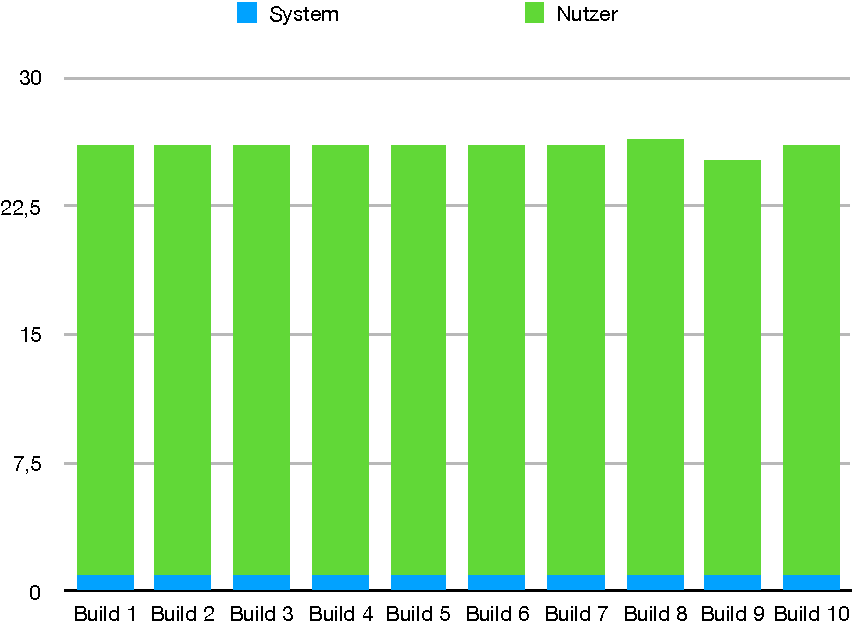
\includegraphics[width=\textwidth]{img/baseline_duration.pdf}
	            \caption{Basismessung | CPU Zeit}
	            \label{figure:baseline_duration}
	        \end{figure}
	        \begin{figure}[p]
	            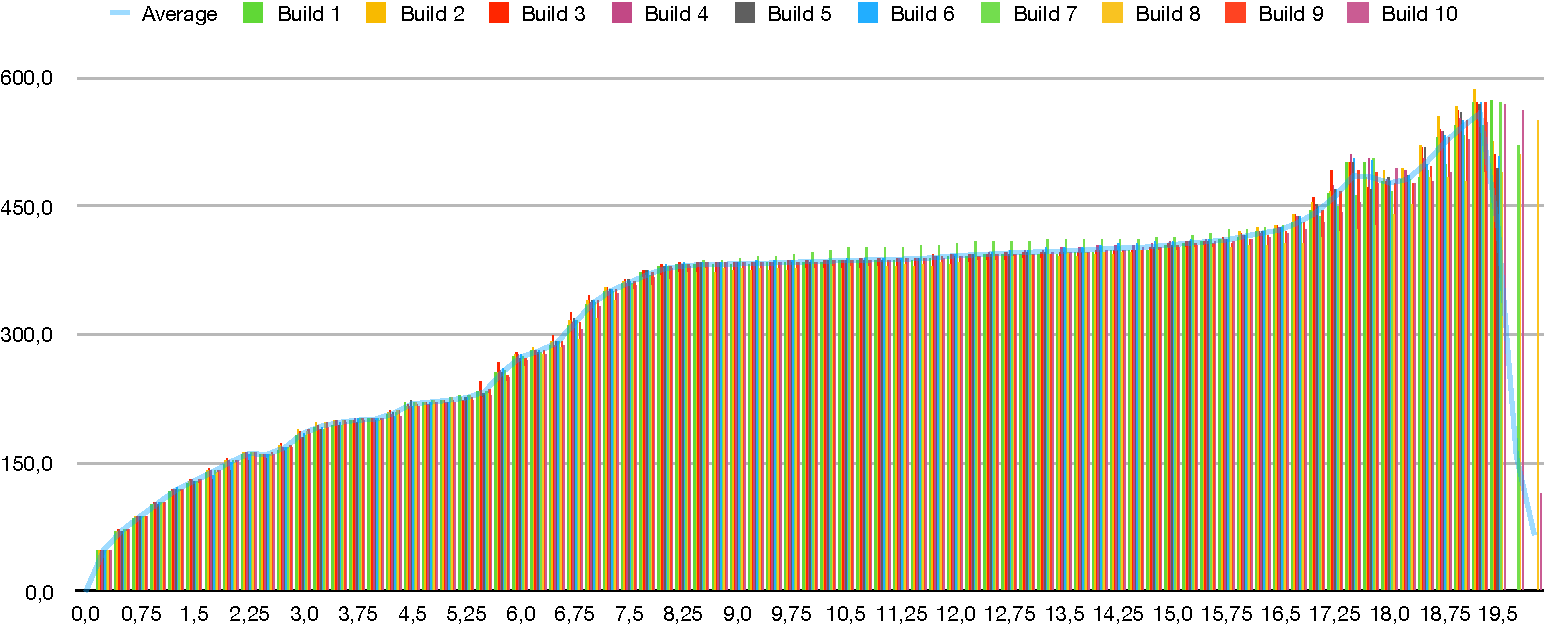
\includegraphics[width=\textwidth]{img/baseline_memory.pdf}
	            \caption{Basismessung | Speicherverbrauch}
	            \label{figure:baseline_memory}
	        \end{figure}

        \section{Nicht destruktive Anpassungen}
        	\label{section:productionOptimizations}
        	\subsection{Optimierung der Minifikation}
        		\label{section:minification}
	        	Das Ersetzen von Leerzeichen und Zeilenumbrüchen einen Großteil der Minifikation aus. Das umstrukturieren von Code hingegen ist zeitaufwändig und bringt vergleichsweise geringe Verbesserungen\cite{optimization-source:minify}.
        		\subsubsection{NoCompress}
        			\label{section:minification_noCompress}
	        		Durch das Deaktivieren der Code-Optimierung wurde die \Gls{cpuTime} um \emph{12,64} Sekunden auf \emph{13,36} Sekunden reduziert. Die Größe der Ausgabedatei hat sich dabei nur um $+2$ Kilobyte auf insgesamt $932$ KB verändert.\\
	        		Abbildung \ref{figure:minification_noCompress_memory} zeigt eine Reduzierung des Speicherverbrauches um ca. $200$ MB.\\
		        	Die Konfigurationsdatei für den Build können auf \href{https://github.com/TexNAK/WebBundlerOptimization/compare/master...nondestr_scopedCompilation#diff-1fb5683b1e7adbcee273b7f9f9a08a22}{GitHub} eingesehen werden.
			        \begin{figure}[p]
			            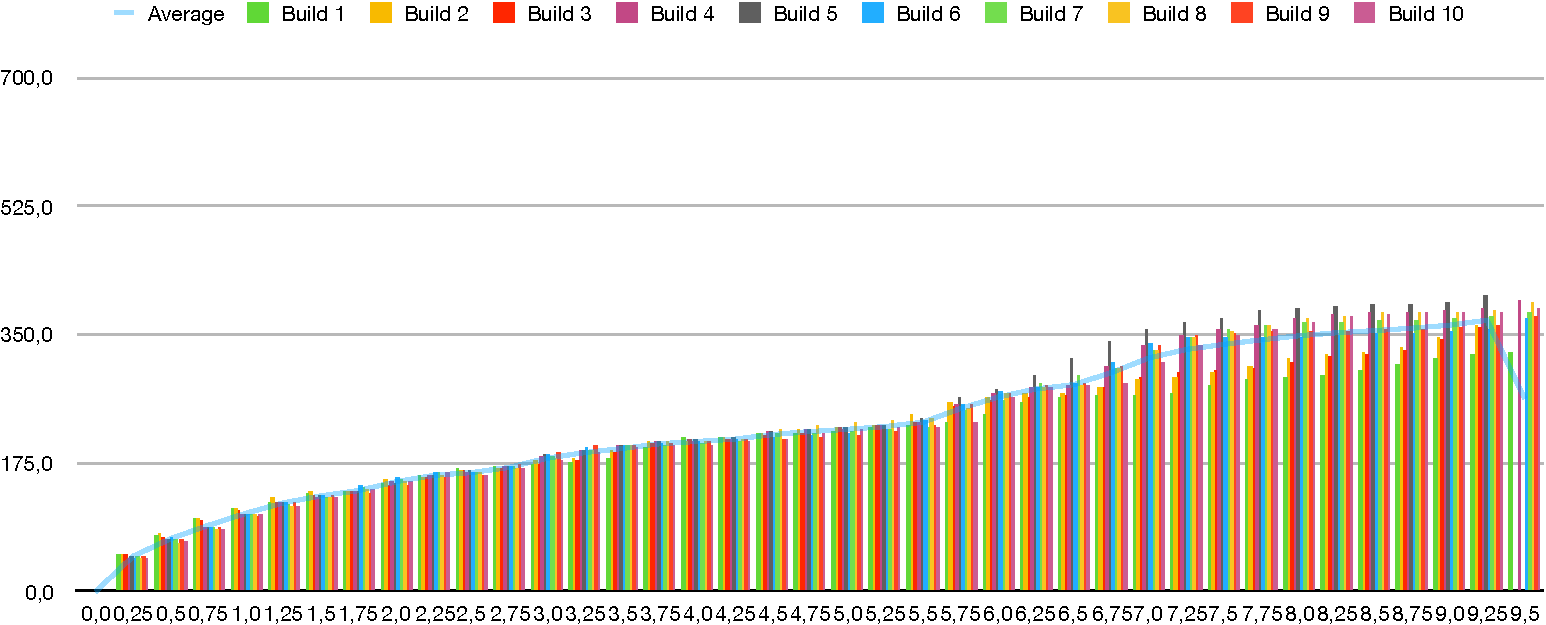
\includegraphics[width=\textwidth]{img/nondestr_minify_nocompress_memory}
			            \caption{Minifikation (noCompress) | Speicherverbrauch}
			            \label{figure:minification_noCompress_memory}
			        \end{figure}

        		\subsubsection{NoMangle}
	        		Durch das Deaktivieren des \Gls{mangling} wurde die \Gls{cpuTime} um \emph{2,66} Sekunden auf \emph{23,34} Sekunden reduziert. Die Größe der Ausgabedatei hat sich dabei um weniger als $1$ KB verändert.\\
	        		Abbildung \ref{figure:minification_noMangle_memory} zeigt eine Reduzierung des Speicherverbrauches um ca. $200$ MB und eine gewisse Varianz in der Laufzeit der einzelnen Buildvorgänge.\\
        			Die Konfigurationsdatei ist großteils identisch mit der in Sektion \ref{section:minification_noCompress} gezeigten mit dem Unterschied, dass statt der Option \emph{compress} die Option \emph{mangle} auf \emph{false} gesetzt wurde.
			        \begin{figure}[p]
			            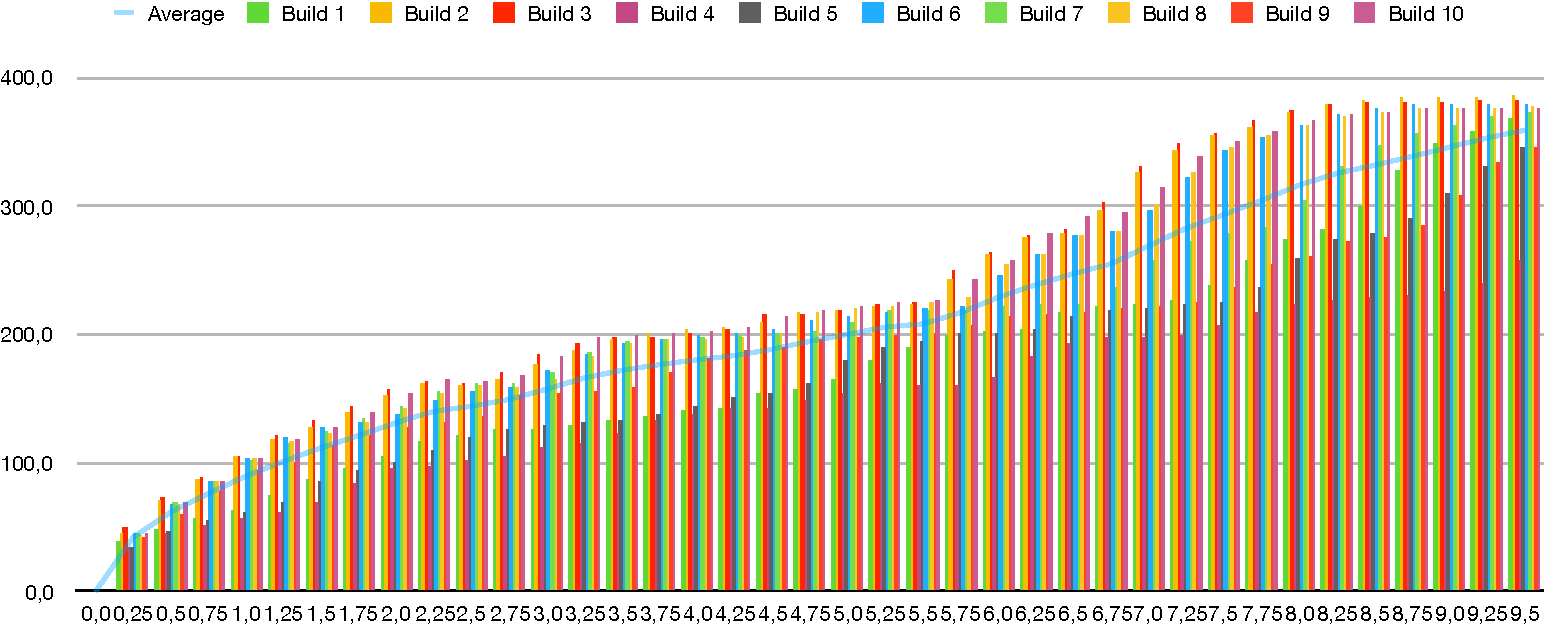
\includegraphics[width=\textwidth]{img/nondestr_minify_nomangle_memory}
			            \caption{Minifikation (noMangle) | Speicherverbrauch}
			            \label{figure:minification_noMangle_memory}
			        \end{figure}

        	\subsection{Scoped compilation}
        		Es ist möglich einen Teil der Abhängigkeiten und auch Teile des Projektes, welche sich nur selten ändern, einmalig zu bauen und in nachfolgenden Builds lediglich einzubinden. Da die meisten Projekte zu einem Großteil aus Abhängigkeiten bestehen\footnote{Ein mit create-react-app v1.5.2 erstelltes Projekt hat 967 Dependencies mit ca. 13.000 JS-Dateien} kann dies zu signifikanten Zeitersparnissen führen. Um die Zeit zu messen wurden folgende Abhängigkeiten in einen extra Build ausgelagert:
        		\begin{itemize}
        			\item react
        			\item react-dom
        			\item @material-ui/core
        			\item @material-ui/icons
        			\item victory
        			\item prop-types
        		\end{itemize}
        		Durch diese Auslagerung wurde die \Gls{cpuTime} des Build dadurch auf \emph{2,93} Sekunden reduziert, was eine Beschleunigung um den Faktor \emph{8,8} gegenüber der Ausgangslage darstellt. Da die größten Abhängigkeiten ausgelagert sind hängt die Dauer des Builds nun lediglich von den eigentlichen Projektdateien ab. Die sehr geringe Zeit lässt sich auf die geringe Größe des Beispiel-Projektes zurückführen. Die reale Zeitersparnis ist somit direkt von der Menge der Abhängigkeiten und Modulen des Projektes ab, welche man in einen extra Build auslagert.\\
        		Ein weiterer Aspekt ist, dass der Speicherverbrauch des Buildprozesses ebenfalls signifikant von maximal $550$ MB auf $150$ MB gesenkt wurde, wie in Abbildung \ref{figure:scopedCompilation_memory} zu sehen ist. Auf Geräten mit geringem Arbeitsspeicher kann dies von Relevanz sein um Swapping und die damit einhergehenden Performanceverluste zu vermeiden.\\
        		Die Konfigurationsdatei für den Build können auf \href{https://github.com/TexNAK/WebBundlerOptimization/compare/master...nondestr_scopedCompilation#diff-1fb5683b1e7adbcee273b7f9f9a08a22}{GitHub} eingesehen werden.

				\begin{figure}[p]
		            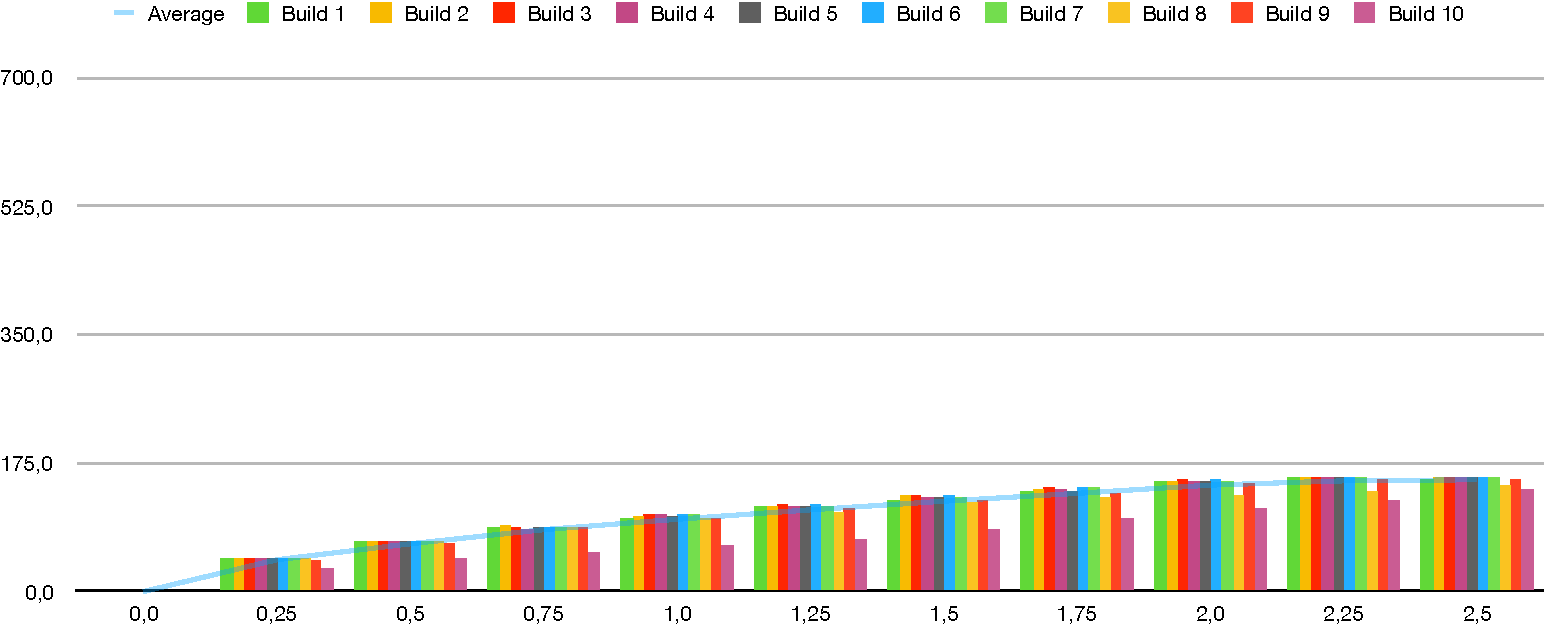
\includegraphics[width=\textwidth]{img/nondestr_scopedCompilation_memory}
		            \caption{Scoped compilation | Speicherverbrauch}
		            \label{figure:scopedCompilation_memory}
		        \end{figure}

    		\subsection{Caching}
    			Es besteht die Möglichkeit die Ausgaben ausgewählter \Gls{loader} zu cachen. In dem Beispiel Projekt macht der \emph{babel-loader} mit ca. \emph{4} Sekunden einen Großteil der Zeit aus, welche von Loadern in Anspruch genommen wird. Daher wurde dieser gecached. Als Resultat wurde die \Gls{cpuTime} auf \emph{22,9} Sekunden reduziert. Abbildung \ref{figure:cache_memory} zeigt eine Reduzierung des Speicherverbrauches um ca. $125$ MB.\\
    			% TODO Push branch and add GitHub Link
    			Die Konfigurationsdatei für den Build können auf \href{INSERTLINKHERE}{GitHub} eingesehen werden.
    			
    			\begin{figure}[p]
		            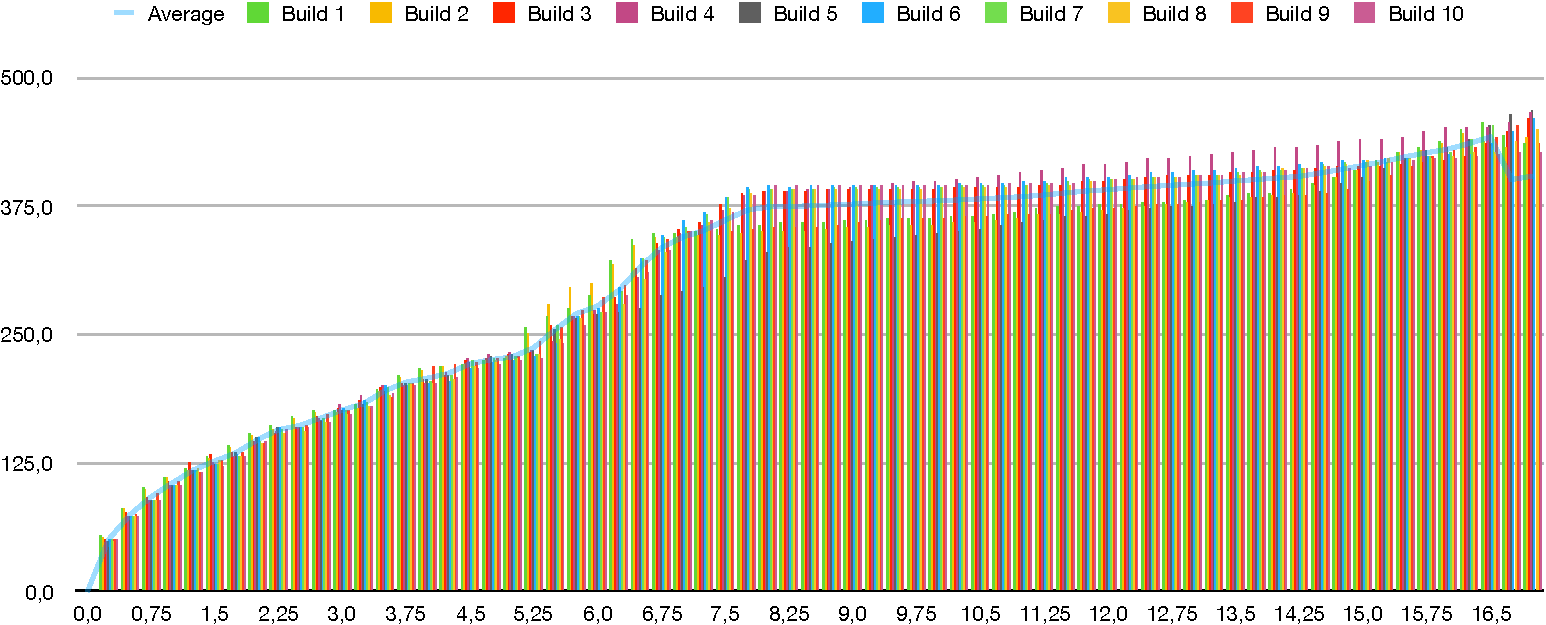
\includegraphics[width=\textwidth]{img/nondestr_cache_memory}
		            \caption{Cache | Speicherverbrauch}
		            \label{figure:cache_memory}
		        \end{figure}

    	\section{Destruktive Anpassungen}
    		\subsection{Source-Maps}
    			Um den Code nach dem Build-Prozess noch debuggen zu können und Stack-Traces für Exceptions mit den entsprechenden Source-Dateien zu verbinden wird eine sogenannte Source-Map gebaut, welche die Relation zwischen den Zeilen in der Ausgabedatei und der Eingabedatei beinhalten. Im Normalfall werden diese Source-Maps für alle Dateien auf Zeilenbasis erzeugt. Es gibt die Möglichkeit die Source-Maps nur auf Modulbasis zu erzeugen. Eine Umstellung auf die modulbasierte Erzeugung resultierte in einer \Gls{cpuTime} von \emph{12} Sekunden. Sofern Source-Maps für die Entwicklung nicht benötigt werden, können sie auch komplett deaktiviert werden.\\
    			Abbildung \ref{figure:sourceMaps_memory} zeigt, dass es keinen signifikanten Unterschied in dem Speicherverbrauch gibt.\\
    			Die Konfigurationsdatei für den Build können auf \href{https://github.com/TexNAK/WebBundlerOptimization/compare/master...destr_cheapSourceMaps#diff-1fb5683b1e7adbcee273b7f9f9a08a22}{GitHub} eingesehen werden.

				\begin{figure}[p]
		            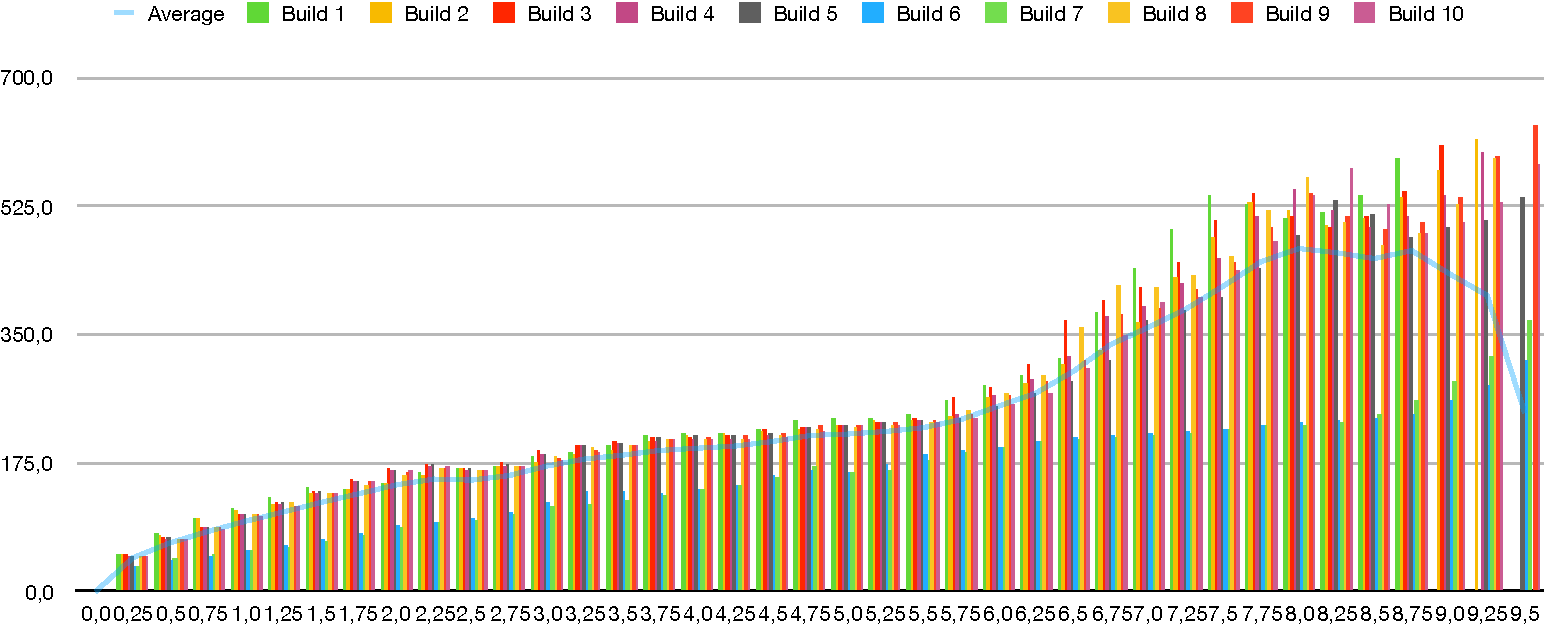
\includegraphics[width=\textwidth]{img/destr_sourceMaps_cheap_memory}
		            \caption{Source Maps (modulbasiert) | Speicherverbrauch}
		            \label{figure:sourceMaps_memory}
		        \end{figure}

    		\subsection{Inkrementelle Builds \& In-Memory-Compilation}
    			\label{section:incrementalBuilds}
    			Normalerweise werden die Ausgabedateien auf die Festplatte geschrieben und bei jedem Build vollständig von vorne erzeugt. Es besteht die Möglichkeit die Ausgabedateien im Speicher zu halten und darauf ausgehend inkrementelle Builds durchzuführen. Im Fall des Beispiel-Projekt wurde dadurch die \Gls{cpuTime} auf \emph{29,99} Sekunden angehoben. Dabei ist zu beachten, dass die \Gls{cpuTime} bei diesen Messungen nicht nur den reinen Build sondern auch die zusätzliche Speicherverwaltung beinhaltet. Außerdem konnte die \Gls{cpuTime} nicht wie in den vorherigen Fällen automatisch gemessen werden sondern wurde manuell dem macOS Activity-Monitor entnommen. Daher ist es leider nicht 

    		\subsection{\Gls{hmr}}
    			Ein weiteres Feature ist das sogenannte \Gls{hmr}. Dies ermöglicht es einen Teil der Website neu zu bauen und das alte Modul in einer offenen Instanz der Seite durch das neue zu ersetzen. Dieses Feature setzt jedoch die in Sektion \ref{section:incrementalBuilds} beschriebene In-Memory-Compilation voraus. Im Durchschnitt nahm der Build \emph{35,42} Sekunden \Gls{cpuTime} in Anspruch.

		\section{Gesamtbewertung}
			\subsection{Umgebungsunabhängig}
				Wenn man sämtliche in Sektion \ref{section:productionOptimizations} beschriebenen Optimierungen in einer Konfiguration zusammenfasst und gemeinsam anwendet, so erreicht man bei dem Beispiel-Projekt eine \Gls{cpuTime} von \emph{2} Sekunden. Da diese Zeit mit der durch Scoped Compilation alleine erreichten Zeit übereinstimmt ist zu vermuten, dass die anderen beschriebenen Optimierungen hauptsächlich die Abhängigkeiten betroffen haben, welche durch Scoped Compilation aus dem Build ausgeschlossen wurden.
			\subsection{Destruktiv}
				Fügt man alle Anpassungen zusammen so erreicht man eine durchschnittliche Build-Zeit von insgesamt \emph{2,6} Sekunden. Da der Build nun aber In-Memory durchgeführt wird, führt der \emph{cache-loader} zu zusätzlichem Overhead, da die Zwischenschritte des Builds auf der Festplatte gespeichert werden. Lässt man diesen aus der Konfiguration raus, so erreicht man eine Zeit von \emph{1,08} Sekunden.

	\chapter{Auswertung}
		Let's hope it got improved! % TODO Evaluate what happened
		\begin{table}[h]
			\centering
            \bgroup
            \def\arraystretch{1.5}
			\begin{tabular}{ l | c | c }
				Optimierung & \Gls{cpuTime} & Speicherverbrauch \\
				\hline
				\hline
				Baseline & 26,00s & 557MB \\
				Minifikation | keine Optimierung & 13,36s & 369MB \\
				Minifikation | kein \Gls{mangling} & 23,34s & 395MB \\
				Scoped compilation & 2,93s & 152MB \\
				Caching & 22,90s & 442MB \\
				Source-Maps (modulbasiert) & 12,00s & 549MB \\
				Inkrementelle In-Memory Builds & 29,99s & --- \\
				\Gls{hmr} & 35,42s & --- \\
				\hline
				Gesamt | Non-Destruktiv & 2,20s & 146MB \\
				Gesamt | Destruktiv & 2,60s & 245MB \\
				Gesamt | Destruktiv (ohne Cache) & 1,08s & 246MB \\
			\end{tabular}
			\egroup
            \caption{Übersicht der Optimierungsresultate}
            \label{table:optimizationResultOverview}
		\end{table}
		
		\section{Beeinflussbarkeit der Build Dauer}
			To be done. Beantwortung der Forschungsfrage \ref{question2} % TODO Write this argument

		\section{Zusammenfassung}
			What have we learned? What haven't we looked at (Multithreading, Code-Splitting, ...) % TODO Write this argument
			
    \pagebreak

    %%%%%%%%%%%%%%
    %% Appendix %%
    %%%%%%%%%%%%%%
    \chapter{Appendix}
	    \hspace{0pt}
    \vfill
    \subsection*{Eidesstattliche Erklärung}
        Hiermit erkläre ich an Eides statt, dass ich die vorliegende Arbeit ohne Hilfe Dritter und ohne Benutzung anderer als der angegebenen Hilfsmittel angefertigt habe. Die aus fremden Quellen direkt oder indirekt übernommenen Gedanken sind als solche kenntlich gemacht. Die Arbeit wurde bisher in gleicher oder ähnlicher Form weder von mir noch von jemand anderem als Prüfungsleistung vorgelegt.
        \vspace{2cm}
        \SignatureAndDate{Unterschrift}
    \vfill
    \hspace{0pt}


    \glsaddall
    \printglossary
    \printglossary[type=\acronymtype]


    \nocite{*}
    \bibliography{main.bib}

\end{document}
